\documentclass{article}
\usepackage{graphicx} %package to manage images
\graphicspath{ {./figures/} }
\usepackage{hyperref}
\usepackage{caption}
\usepackage[font=scriptsize]{subcaption}
\captionsetup[figure]{labelsep=none}
\captionsetup[table]{labelsep=none}
\usepackage{bbm}
\usepackage{amsmath}
\usepackage{import}
\usepackage{array}
\usepackage{booktabs}
\usepackage{afterpage}
\usepackage{floatrow}
\usepackage{pdflscape}
\usepackage{soul}
\usepackage{float}
\usepackage{adjustbox}
\usepackage{longtable}


\title{maternal nutrition by social group}

\date{June 2025}

\begin{document}

\maketitle


\section{BMI : 5 covariates reweighting, single year age bins }

reweighting vars used: age edu rural hasboy c user

\begin{table}[H]
    \centering
    \footnotesize % shrink text
    \caption{: BMI by group, reweighting vars used: age edu rural hasboy c user}
    \label{tab:sumstat}
    \adjustbox{width=\textwidth}{\begin{tabular}{lccc}
\toprule
Group & BMI & \% pregnant sample dropped \\\\
\midrule
Forward: parity 0&22.7 (22.4, 22.9)&.14\\
Forward: parity 1&22.8 (22.6, 23.1)&.09\\
Forward: parity 2&22.6 (22.3, 22.9)&0\\
Forward: parity 3&23.0 (22.3, 23.6)&5.33\\
Forward: parity 4+&22.8 (22.0, 23.5)&4.44\\
OBC: parity 0&21.8 (21.7, 21.9)&.06\\
OBC: parity 1&22.1 (22.0, 22.2)&.04\\
OBC: parity 2&21.9 (21.8, 22.1)&0\\
OBC: parity 3&21.6 (21.4, 21.8)&.91\\
OBC: parity 4+&21.0 (20.4, 21.7)&2.82\\
Dalit: parity 0&21.7 (21.6, 21.9)&0\\
Dalit: parity 1&21.9 (21.8, 22.1)&.25\\
Dalit: parity 2&21.8 (21.6, 21.9)&.14\\
Dalit: parity 3&21.4 (21.1, 21.6)&.36\\
Dalit: parity 4+&21.4 (21.1, 21.7)&2.48\\
Adivasi: parity 0&20.9 (20.7, 21.2)&.26\\
Adivasi: parity 1&22.5 (20.1, 24.9)&.06\\
Adivasi: parity 2&21.1 (20.8, 21.4)&.11\\
Adivasi: parity 3&20.8 (20.3, 21.3)&.5\\
Adivasi: parity 4+&20.7 (20.1, 21.3)&.32\\
Muslim: parity 0&22.3 (22.1, 22.5)&.07\\
Muslim: parity 1&22.8 (22.5, 23.1)&.1\\
Muslim: parity 2&22.9 (22.7, 23.1)&.56\\
Muslim: parity 3&23.0 (22.2, 23.7)&.42\\
Muslim: parity 4+&22.8 (22.0, 23.5)&.85\\
\bottomrule
\end{tabular}
}
\end{table}


\section{underweight : 5 covariates reweighting, single year age bins }

reweighting vars used: age edu rural hasboy c user

\begin{table}[H]
    \centering
    \footnotesize % shrink text
    \caption{: Underweight by group, reweighting vars used: age edu rural hasboy c user}
    \label{tab:sumstat}
    \adjustbox{width=\textwidth}{\begin{tabular}{lccc}
\toprule
Group & \% underweight & \% pregnant sample dropped \\\\
\midrule
Forward: parity 0&0.1 (0.1, 0.2)&.14\\
Forward: parity 1&0.1 (0.1, 0.2)&.09\\
Forward: parity 2&0.1 (0.1, 0.2)&0\\
Forward: parity 3&0.1 (0.1, 0.2)&5.33\\
Forward: parity 4+&0.1 (0.0, 0.2)&4.44\\
OBC: parity 0&0.2 (0.2, 0.2)&.06\\
OBC: parity 1&0.2 (0.2, 0.2)&.04\\
OBC: parity 2&0.2 (0.2, 0.2)&0\\
OBC: parity 3&0.2 (0.2, 0.2)&.91\\
OBC: parity 4+&0.2 (0.1, 0.4)&2.82\\
Dalit: parity 0&0.2 (0.2, 0.2)&0\\
Dalit: parity 1&0.2 (0.2, 0.2)&.25\\
Dalit: parity 2&0.2 (0.2, 0.2)&.14\\
Dalit: parity 3&0.2 (0.2, 0.2)&.36\\
Dalit: parity 4+&0.2 (0.2, 0.2)&2.48\\
Adivasi: parity 0&0.2 (0.2, 0.3)&.26\\
Adivasi: parity 1&0.2 (0.1, 0.2)&.06\\
Adivasi: parity 2&0.2 (0.2, 0.3)&.11\\
Adivasi: parity 3&0.3 (0.2, 0.4)&.5\\
Adivasi: parity 4+&0.3 (0.2, 0.4)&.32\\
Muslim: parity 0&0.1 (0.1, 0.1)&.07\\
Muslim: parity 1&0.1 (0.1, 0.1)&.1\\
Muslim: parity 2&0.1 (0.1, 0.1)&.56\\
Muslim: parity 3&0.1 (0.1, 0.1)&.42\\
Muslim: parity 4+&0.1 (0.1, 0.2)&.85\\
\bottomrule
\end{tabular}
}
\end{table}


\section{bmi : 5 covariates reweighting, 2 year age bins }

reweighting vars used: age edu rural hasboy c user

\begin{table}[H]
    \centering
    \footnotesize % shrink text
    \caption{: Underweight by group, reweighting vars used: age edu rural hasboy c user}
    \label{tab:sumstat}
    \adjustbox{width=\textwidth}{\begin{tabular}{lccc}
\toprule
Group & \% underweight & \% pregnant sample dropped \\\\
\midrule
Forward: parity 0&0.1 (0.1, 0.2)&.14\\
Forward: parity 1&0.1 (0.1, 0.2)&.09\\
Forward: parity 2&0.1 (0.1, 0.2)&0\\
Forward: parity 3&0.1 (0.1, 0.2)&5.33\\
Forward: parity 4+&0.1 (0.0, 0.2)&4.44\\
OBC: parity 0&0.2 (0.2, 0.2)&.06\\
OBC: parity 1&0.2 (0.2, 0.2)&.04\\
OBC: parity 2&0.2 (0.2, 0.2)&0\\
OBC: parity 3&0.2 (0.2, 0.2)&.91\\
OBC: parity 4+&0.2 (0.1, 0.4)&2.82\\
Dalit: parity 0&0.2 (0.2, 0.2)&0\\
Dalit: parity 1&0.2 (0.2, 0.2)&.25\\
Dalit: parity 2&0.2 (0.2, 0.2)&.14\\
Dalit: parity 3&0.2 (0.2, 0.2)&.36\\
Dalit: parity 4+&0.2 (0.2, 0.2)&2.48\\
Adivasi: parity 0&0.2 (0.2, 0.3)&.26\\
Adivasi: parity 1&0.2 (0.1, 0.2)&.06\\
Adivasi: parity 2&0.2 (0.2, 0.3)&.11\\
Adivasi: parity 3&0.3 (0.2, 0.4)&.5\\
Adivasi: parity 4+&0.3 (0.2, 0.4)&.32\\
Muslim: parity 0&0.1 (0.1, 0.1)&.07\\
Muslim: parity 1&0.1 (0.1, 0.1)&.1\\
Muslim: parity 2&0.1 (0.1, 0.1)&.56\\
Muslim: parity 3&0.1 (0.1, 0.1)&.42\\
Muslim: parity 4+&0.1 (0.1, 0.2)&.85\\
\bottomrule
\end{tabular}
}
\end{table}


\section{underweight : 5 covariates reweighting, 2 year age bins }

reweighting vars used: age edu rural hasboy c user

\begin{table}[H]
    \centering
    \footnotesize % shrink text
    \caption{: Underweight by group, reweighting vars used: age edu rural hasboy c user}
    \label{tab:sumstat}
    \adjustbox{width=\textwidth}{\begin{tabular}{lccc}
\toprule
Group & \% underweight & \% pregnant sample dropped \\\\
\midrule
Forward: parity 0&0.1 (0.1, 0.2)&.14\\
Forward: parity 1&0.1 (0.1, 0.2)&.09\\
Forward: parity 2&0.1 (0.1, 0.2)&0\\
Forward: parity 3&0.1 (0.1, 0.2)&5.33\\
Forward: parity 4+&0.1 (0.0, 0.2)&4.44\\
OBC: parity 0&0.2 (0.2, 0.2)&.06\\
OBC: parity 1&0.2 (0.2, 0.2)&.04\\
OBC: parity 2&0.2 (0.2, 0.2)&0\\
OBC: parity 3&0.2 (0.2, 0.2)&.91\\
OBC: parity 4+&0.2 (0.1, 0.4)&2.82\\
Dalit: parity 0&0.2 (0.2, 0.2)&0\\
Dalit: parity 1&0.2 (0.2, 0.2)&.25\\
Dalit: parity 2&0.2 (0.2, 0.2)&.14\\
Dalit: parity 3&0.2 (0.2, 0.2)&.36\\
Dalit: parity 4+&0.2 (0.2, 0.2)&2.48\\
Adivasi: parity 0&0.2 (0.2, 0.3)&.26\\
Adivasi: parity 1&0.2 (0.1, 0.2)&.06\\
Adivasi: parity 2&0.2 (0.2, 0.3)&.11\\
Adivasi: parity 3&0.3 (0.2, 0.4)&.5\\
Adivasi: parity 4+&0.3 (0.2, 0.4)&.32\\
Muslim: parity 0&0.1 (0.1, 0.1)&.07\\
Muslim: parity 1&0.1 (0.1, 0.1)&.1\\
Muslim: parity 2&0.1 (0.1, 0.1)&.56\\
Muslim: parity 3&0.1 (0.1, 0.1)&.42\\
Muslim: parity 4+&0.1 (0.1, 0.2)&.85\\
\bottomrule
\end{tabular}
}
\end{table}



% \section{outcome: BMI}
% \begin{figure}[H]
%     \centering
%     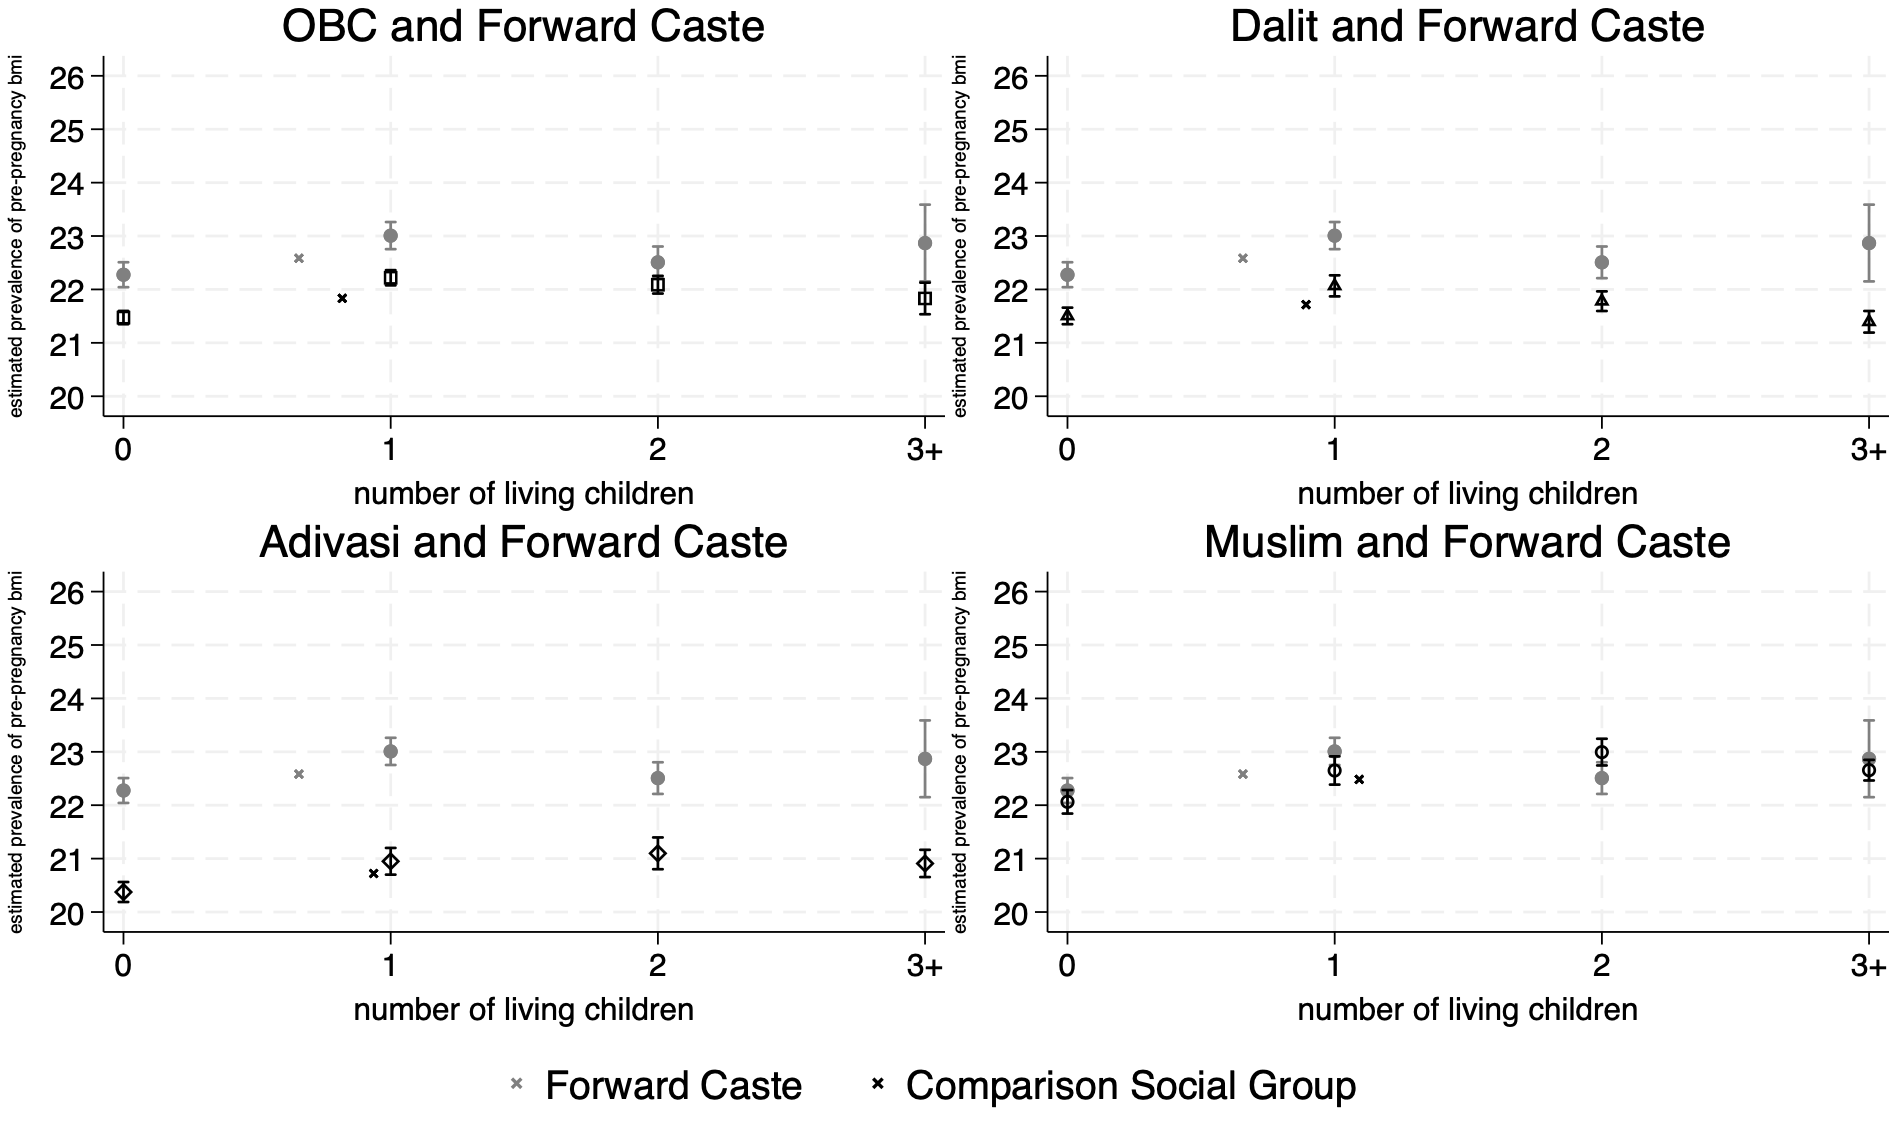
\includegraphics[width=\textwidth]{figures/prepreg_bmi_combined.png}
% \end{figure}

% \section{outcome: underweight}
% \begin{figure}[H]
%     \centering
%     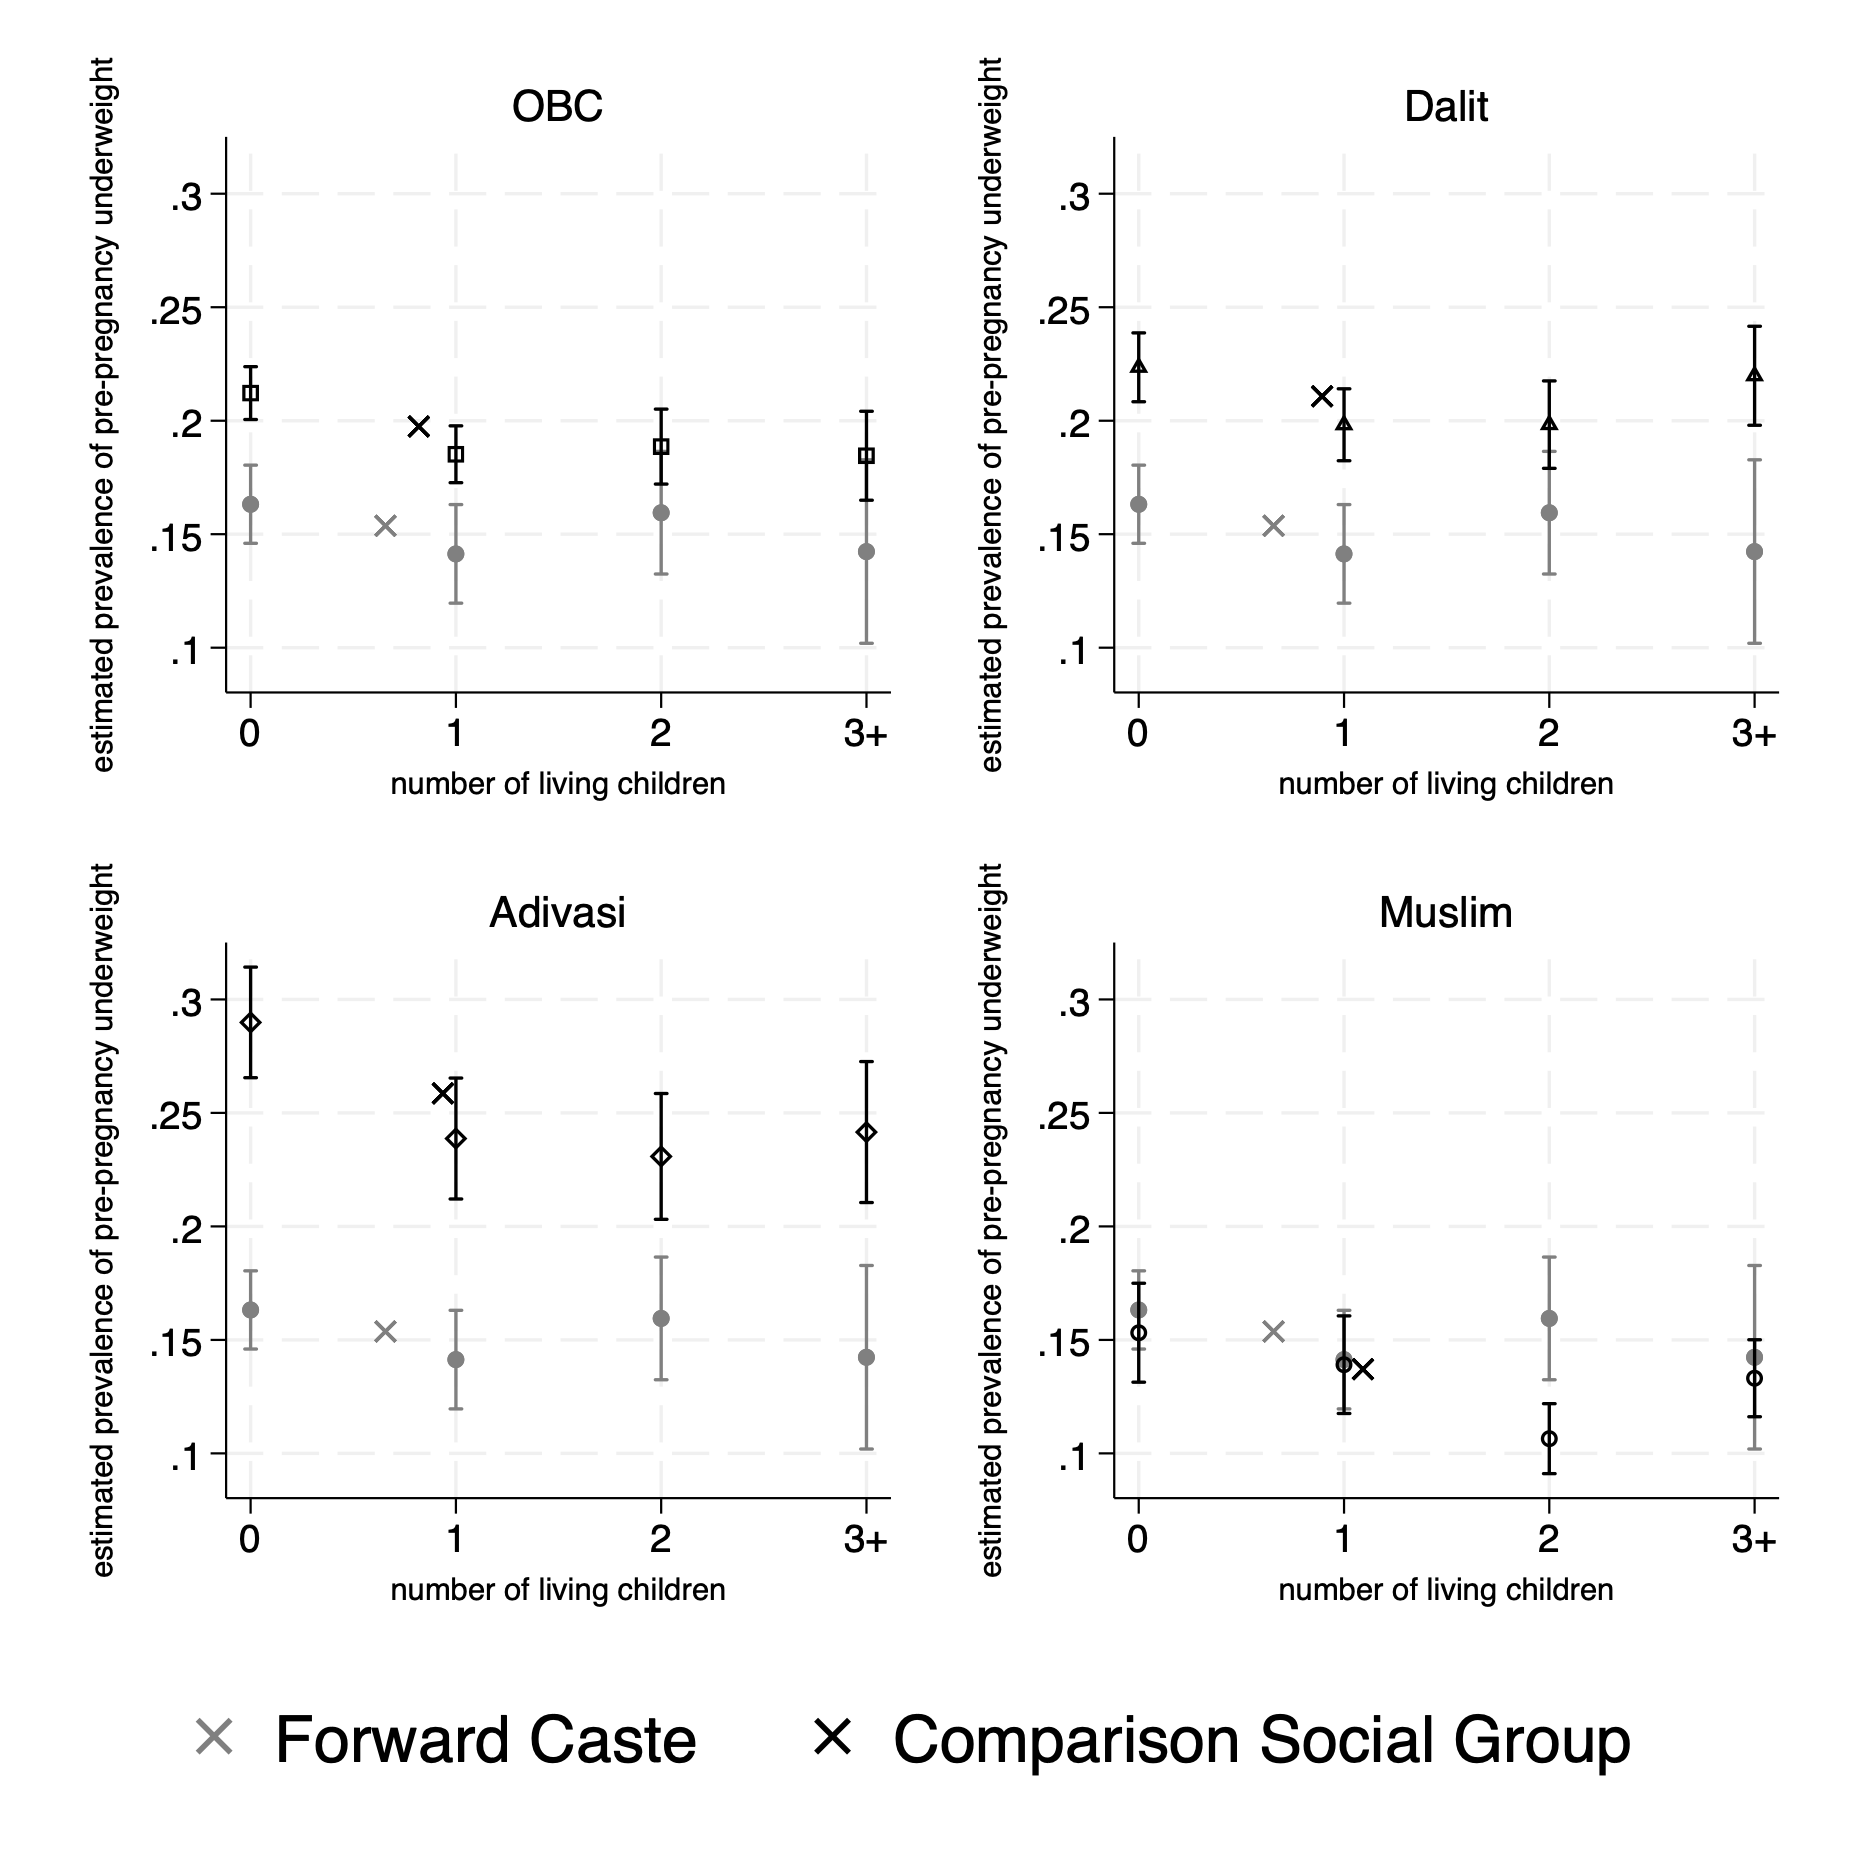
\includegraphics[width=\textwidth]{figures/prepreg_underweight_combined.png}
% \end{figure}

% \section{stacked bar graph}
% \begin{figure}[H]
%     \centering
%     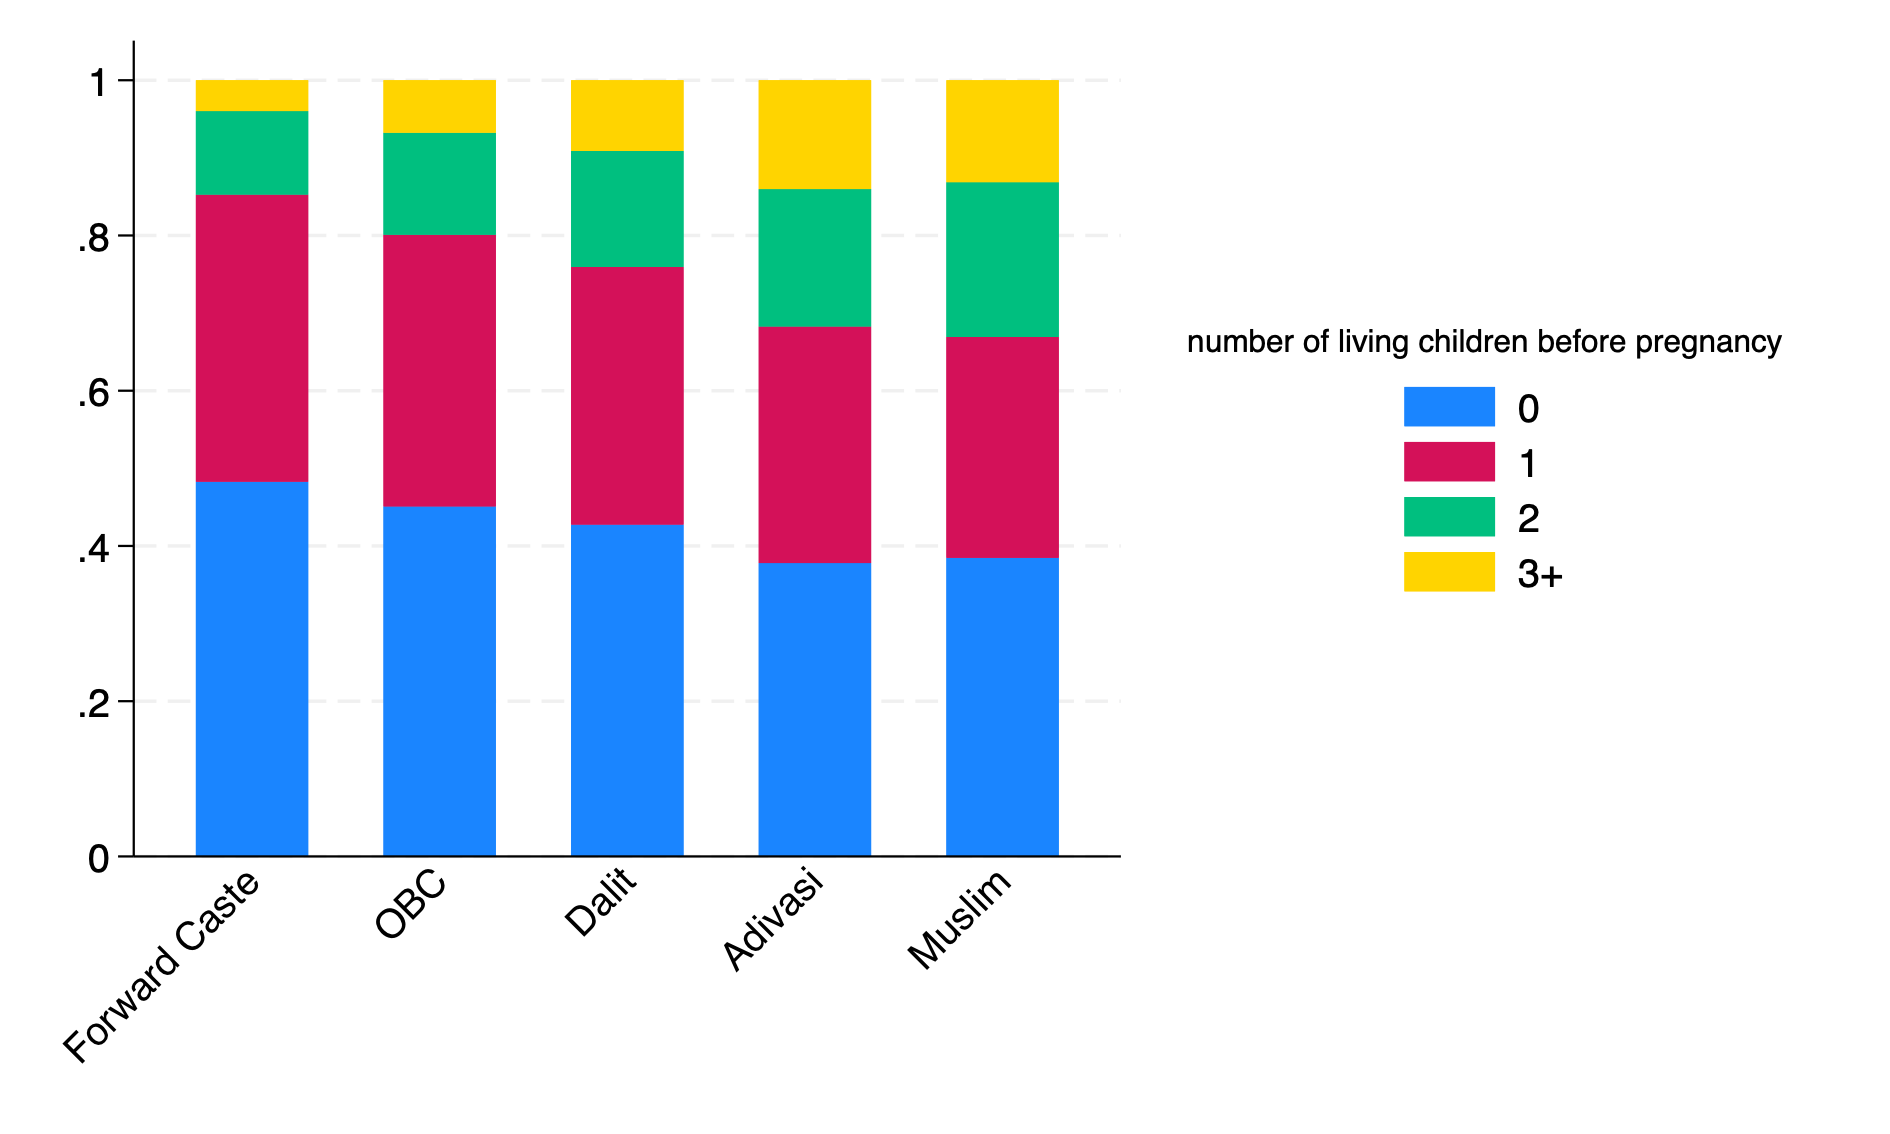
\includegraphics[width=\textwidth]{figures/stackedbar_parity_socialgroup.png}
% \end{figure}




\end{document}
